%! suppress = Makeatletter
%! suppress = Makeatletter
\documentclass[11pt]{report}

\usepackage[T1]{fontenc}
\usepackage[utf8]{inputenc}
\usepackage{graphicx}
\usepackage{amsmath,amssymb,amsfonts}
\usepackage{polski}
\usepackage[raggedright]{titlesec}
\usepackage{indentfirst}
\usepackage{listings}
\usepackage{hyperref}
\usepackage[backend=biber, bibencoding=utf8, style=ieee, dashed=false, isbn=false, doi=false, sorting=anyvt]{biblatex}

\addbibresource{library.bib}

\pagestyle{headings}

\renewcommand{\chaptername}{Rozdział}
\renewcommand{\contentsname}{Spis treści}
\renewcommand{\figurename}{Rys.}
\renewcommand{\tablename}{Tab.}
\renewcommand{\listfigurename}{Spis rysunków}
\renewcommand{\listtablename}{Spis tabel}
\renewcommand{\bibname}{Bibliografia}

\makeatletter
\renewcommand{\l@section}{\@dottedtocline{1}{1.5em}{2.6em}}
\renewcommand{\l@subsection}{\@dottedtocline{2}{4.0em}{3.6em}}
\renewcommand{\l@subsubsection}{\@dottedtocline{3}{7.4em}{4.5em}}
\makeatother


\begin{document}

    \begin{titlepage}
        \centering
        
\includegraphics[width=1 \textwidth]{fig/AGH.jpg}
        \center{\scshape WYDZIAŁ INFORMATYKI, ELEKTRONIKI\\ I TELEKOMUNIKACJI\\
        Kierunek Informatyka}
        \vspace{0.03\textheight}
        \center{\scshape Michał Patyk}
        \bigskip
        \center{\LARGE\bfseries Analiza danych i wzorców dotyczących wydarzeń politycznych na podstawie informacji zgromadzonych w projekcie GDELT}
        \center{(pracownia problemowa)}
        \vspace{0.2\textheight}
        \par
        \rightline{Opiekun: dr hab. inż. Koźlak Jarosław}

        \vspace{0.1\textheight}
        \center{Kraków 2020}
    \end{titlepage}

    \tableofcontents


    \chapter{Wstęp}
    //Wydarzenia są opisywane przez zaangażowanych aktorów (którymi mogą być państwa lub specyficzne organizacje) oraz lokalizacje i kategorie definiujące charakter wydarzeń (np. różne rodzaje negocjacji , deklaracji politycznych, zamieszki, konflikty zbrojne, itp.), co jest specyfikowane przez zestawy szczegółowych atrybutów.

    //Postawić problem
    //dlaczego chemy realizować
    //na podstawie analiz chcemy lepiej zrozumieć specyfikę krajów
    //chęć automatycznej reakcji na to że cos sie dzieje
    //informacja o zdarzeniach nietypowych
    //jak społeczności reagują
    //patrz dyplom KKI


    \section{Cele pracy}
    Celem niniejszej pracy jest analiza wydarzeń politycznych oraz poszukiwanie występujących w nich wzorców w oparciu o dane projektu GDELT.


    \chapter{Przegląd dziedziny}
    W tym rozdziale opisany został zbiór danych GDELT, schemat kodwania CAMEO oraz przeprowadzony został przegląd istniejących analiz zbioru.


    \section{GDELT}
    GDELT - Global Database of Events, Language, and Tone - to największa, najbardziej wszechstronna i otwarta baza danych jaka powstała.
    Wczesne poszukiwania prowadzące do stworzenia GDELT zostały opisane przez Philipa Schrodta w dokumencie~\cite{Schrodt2010} w styczniu 2010 r.
    Zbiór danych jest dostępny na stronie Projektu ~\cite{gdelt} oraz na platformie Google Cloud gdzie można z niego korzystać przez Google BigQuery~\cite{BigQuery2014}.
    GDELT używa kodowania obserwacji konfliktów i mediacji (CAMEO)~\cite{GDELTDocumentation} do rejestrowania zdarzeń.
    W zbiorze znajdują się dane od 1979 roku.
    Kolejne porcje zdarzeń i ich klasyfikacja generowane sa na bieżąco każdego dnia.


    \section{CAMEO}
    CAMEO - Conflict and Mediation Event Observations - jest schematem kodowania zdarzeń.
    Został stworzony w Katedrze Nauk Politycznych Pennsylvania State University.
    Jego początki sięgają roku 2000.
    Został zaprojektowany z myślą o automatycznym kodowaniu i szczegółowym kodowaniu aktorów.

    \subsection{Zdarzenia}
    Kody zdarzeń są ujednolicone pod względem kolejności numerycznej głównych kategorii.
    Kategorie są uszeregowane rosnąco względem kooperacji od 01 do 09 oraz względem konfliktu od 10 do 20.

    \subsection{Aktorzy}
    Kody aktorów składają sie z trzech znaków.
    Elementy kodu są podzielone na szerokie kategorie, takie jak podmioty państwowe, role, regiony i grupy etniczne aktorów.


    \section{Przegląd istniejących analiz} \label{ch:przeglad}
    // artykuły analizujące, kto cytował, jakie analizy


    \chapter{Koncepcja}
    // jaki system chcemy stworzyć
    // wektory, algorytmy klastrowania

    W tym rozdziale zostały opisane\ldots


    \section{Założenia i wymagania}
    W analizie wykorzystany zostanie głównie zbiór danych GDELT 2.0 od początku 2015 roku do kwietnia 2020.


    \section{Efekt końcowy}
    Planowanym efektem końcowym pracy będzie\ldots


    \chapter{Realizacja}


    \section{Wykorzystane narzędzia}

    \begin{enumerate}
        \item[•] język programowania Python~\cite{python}
        \item[•] biblioteka Pandas~\cite{pandas}
        \item[•] biblioteka GeoPandas~\cite{geopandas}
        \item[•] biblioteka Scikit-Learn~\cite{scikit}
        \item[•] środowisko programistyczne PyCharm~\cite{pycharm}
        \item[•] internetowe interaktywne środowisko obliczeniowe Notebook Jupyter~\cite{jupyter}
        \item[•] hurtownia danych Google BigQuery~\cite{bigquery}
    \end{enumerate}

    // dyskusja co można by wykorzystac zamiast tych narzędzi np dane lokalne zamiast bigQuery

    Przy tworzniu projektu wykorzystany został język programowania Python.
    Jest to język wysokiego poziomu ogólnego przeznaczenia.
    Wraz z biblioteka Pandas jest często stosowany w zagadnieniach analizy danych oraz data miningu.
    Głównym narzędziem używanym do programowania było zintegrowane środowisko programistyczne PyCharm firmy JetBrains.
    Pozwala ono na wygodną edycję i analizę kodu źródłowego.
    Internetowe interaktywne środowisko obliczeniowe Notebook Jupyter pozwoliło na tworzenie dokumentów zawierających kod wraz z wizualizacjami.
    Wykorzystanie hurtowni danych Google BigQuery pozwoliło na szybką, skalowalną analizę dużego zbioru danych jakim jest GDELT.
    BigQuery jest oprogramowaniem bezserwerowym, które obsługuje zapytania w języku ANSI SQL.
    Podział krajów na klastry został wykonany przy użyciu Scikit-Learn.
    Do wizualizacji klastrów na mapie wykorzystano bibliotekę GeoPandas.


    \section{Wstępna analiza danych}
    W tej części pracy przeprowadzona zostanie wstępna analiza zagregowanych danych. W pierwszej kolejności przeanalizowane zostaną dane dotyczące Polski, co pozwoli na łatwiejsze wychwycenie związków między zarejestrowanymi wydarzeniami, a sytuacją w kraju.
    W dalszej kolejności przeprowadzona zostania analiza zbiorcza dla wszystkich krajów.

    \subsection{Popularność Polski w zbiorze danych GDELT}
    Jako pierwszą analizę wykonano badanie popularności Polski w zbiorze danych GDELT. Na wszystkich trzech wykresach obserwujemy znaczny wzrost ilości zdarzeń w 2015 roku. Może być to związane z uruchomieniem w GDELT automatycznego tłumaczenia artykułów i co za tym idzie zwiększeniem ilości źródeł danych.

    \paragraph{Polska jako Aktor 1}
    Wykers~\ref{fig:PLactor1} przedstawia popularność Polski jako aktora 1 skumulowaną dla poszczególnych lat.
    W roku 2016 obserwujemy szczyt popularności na poziomie około 150 tysięcy zdarzeń.
    \begin{figure}[ht]
        \centering
        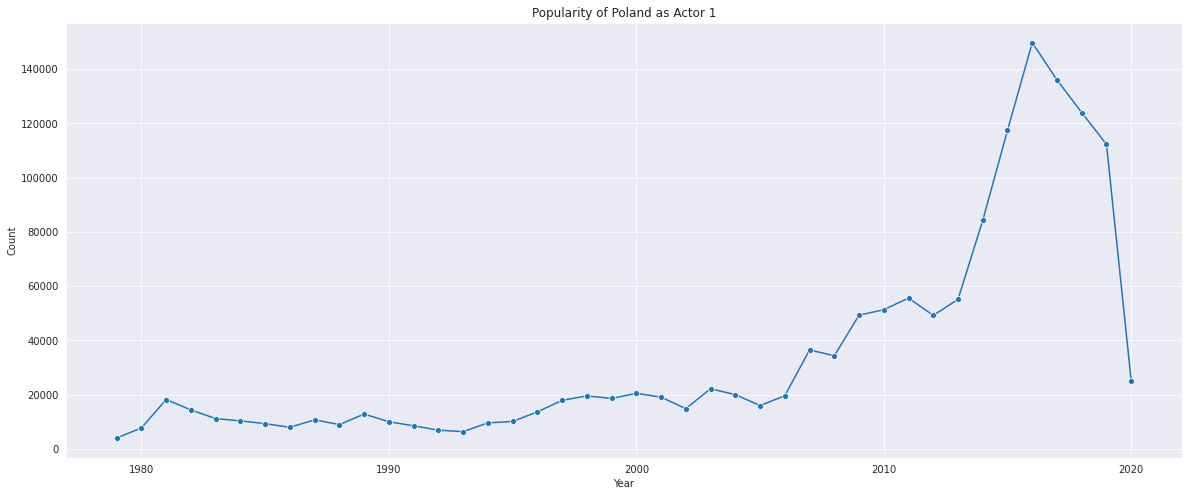
\includegraphics[width=1 \textwidth]{fig/PL/PLactor1.png}
        \caption{Ilość zdarzeń z Polską jako aktorem 1. (zródło: opracowanie własne)}
        \label{fig:PLactor1}
        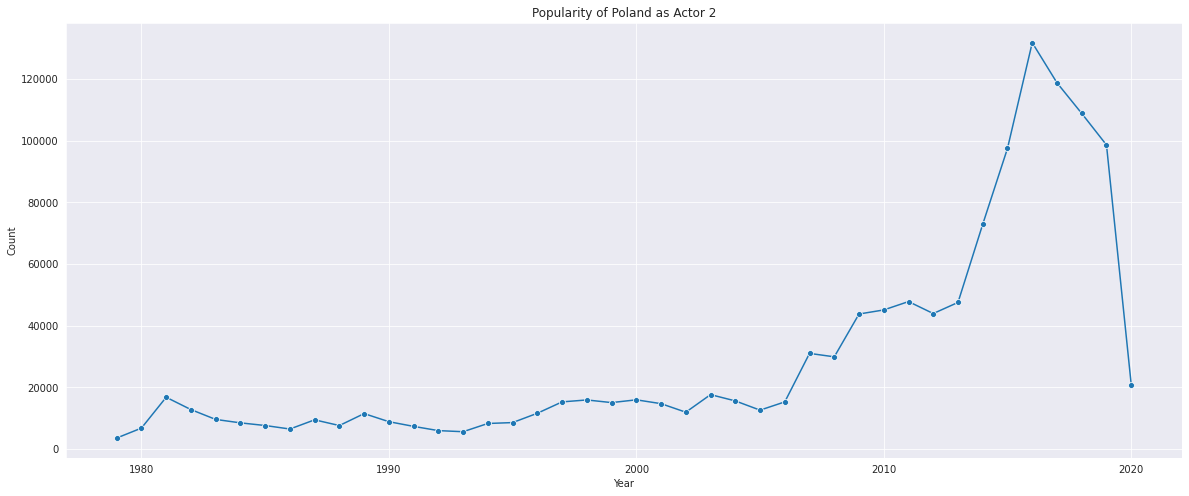
\includegraphics[width=1 \textwidth]{fig/PL/PLactor2.png}
        \caption{Ilość zdarzeń z Polską jako aktorem 2. (zródło: opracowanie własne)}
        \label{fig:PLactor2}
    \end{figure}

    \paragraph{Polska jako Aktor 2}
    Wykers~\ref{fig:PLactor2} przedstawia popularność Polski jako aktora 2 skumulowaną dla poszczególnych lat. Kształt wykresu jest bardzo zbliżony do~\ref{fig:PLactor1} jednak szczyt popularności jest niższy - na poziomie około 130 tysięcy zdarzeń.

    \paragraph{Polska jako miejsce wydarzeń}
    Wykers~\ref{fig:PLlocation} przedstawia popularność Polski jako miejsca wydarzeń skumulowaną dla poszczególnych lat. Ponownie kształt wykresu jest zbliżony do~\ref{fig:PLactor1}. W tym przypadku szczyt popularności jest wyższy - na poziomie około 210 tysięcy zdarzeń.
    \begin{figure}[ht]
        \centering
        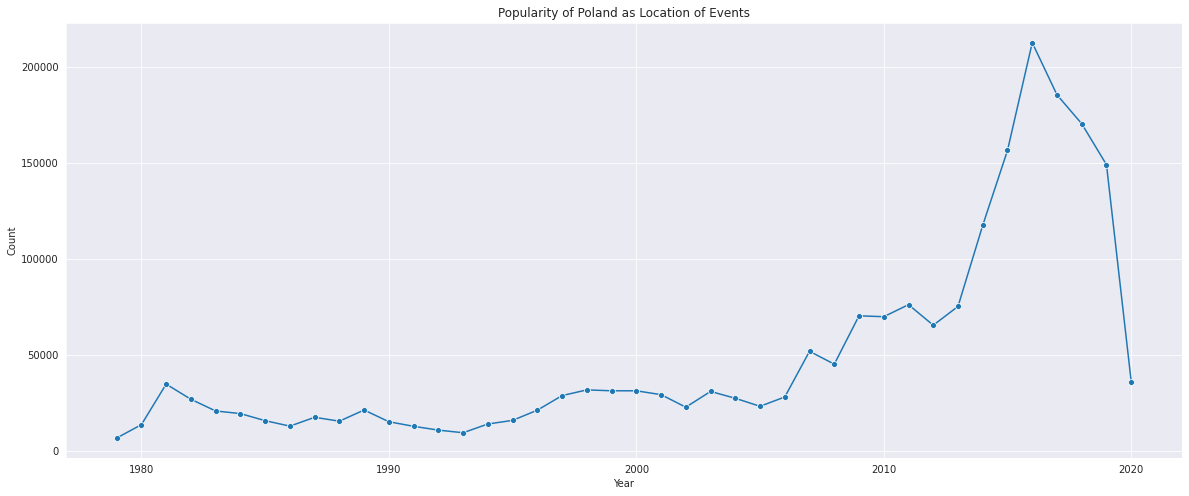
\includegraphics[width=1 \textwidth]{fig/PL/PLlocation.png}
        \caption{Ilość zdarzeń z Polską jako lokacją. (zródło: opracowanie własne)}
        \label{fig:PLlocation}
    \end{figure}

    \subsection{Analiza zbiorcza od 2015 roku}
    Dane pochodzą z przedziału od stycznia 2015 do kwietnia 2020 roku.

    \paragraph{Ilość zdarzeń dla poszczególnych krajów}
    Wykres~\ref{fig:GLOBALactor1} przedstawia sumaryczną ilość zdarzeń od 2015 roku, dla poszczególnych krajów, uszeregowaną malejąco.
    \begin{figure}[ht]
        \centering
        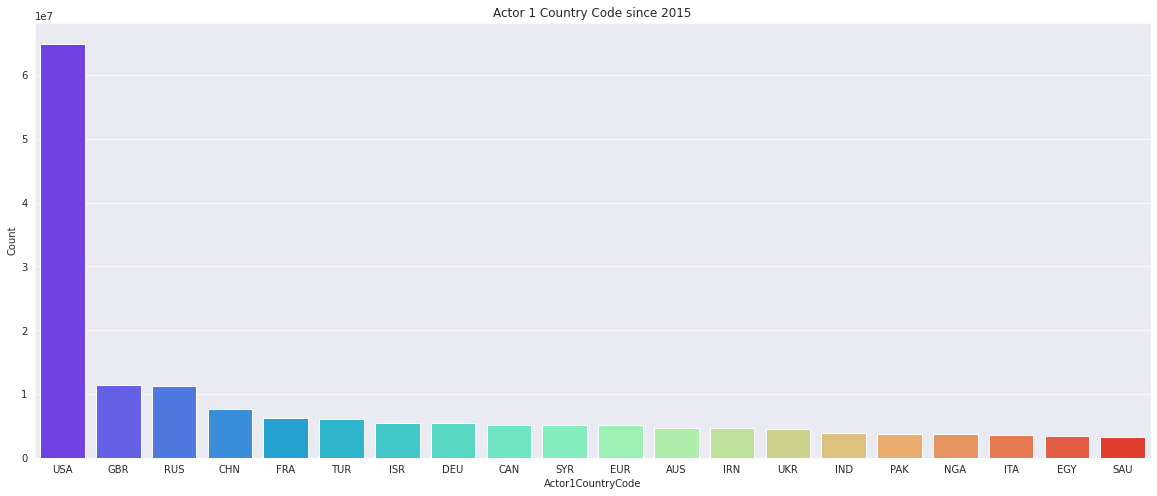
\includegraphics[width=1 \textwidth]{fig/GLOBAL/Actor1.png}
        \caption{Ilość zdarzeń dla poszczególnych krajów. (zródło: opracowanie własne)}
        \label{fig:GLOBALactor1}
    \end{figure}
    Niekwestionowanym liderem pod względem ilości zdarzeń są Stany Zjednoczone. Dystansują one pozostałe kraje o prawie rząd wielkości. Kraje anglosaskie są szczeegolnie mocno reprezentowane. W czołówce pojawiają sie też kraje znaczace polictycznie oraz silnie skonfliktowane.

    \paragraph{Ilość zdarzeń w czasie}
    Wykres~\ref{fig:GLOBALactor1inTime} przedstawia ilość zdarzeń dla top 5 krajów skumulowaną dla poszczególnych lat.
    WYKRES DO POPRAWY
    \begin{figure}[ht]
        \centering
        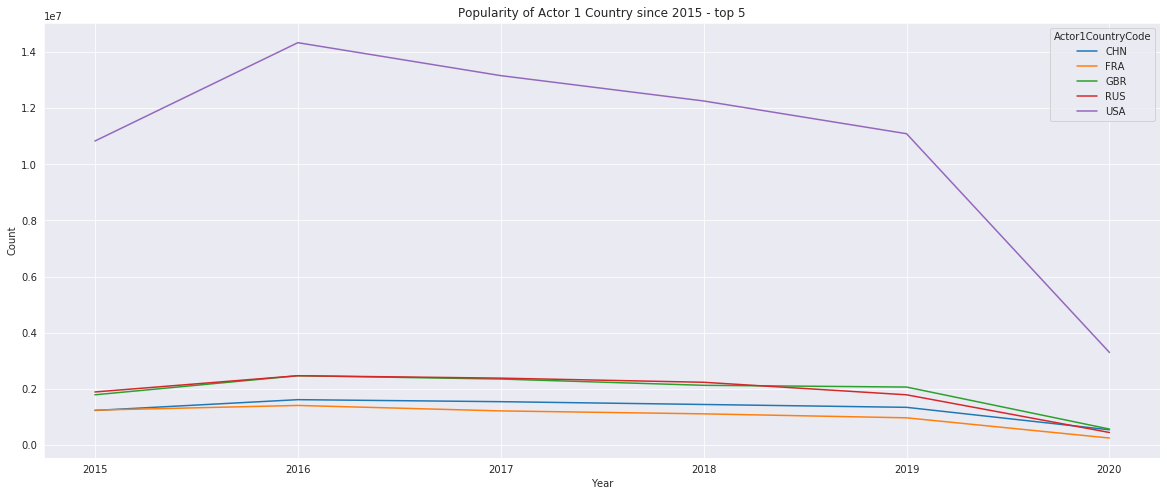
\includegraphics[width=1 \textwidth]{fig/GLOBAL/Actor1inTIME.png}
        \caption{Ilość zdarzeń dla poszczególnych krajów w czasie. (zródło: opracowanie własne)}
        \label{fig:GLOBALactor1inTime}
    \end{figure}

    \paragraph{Popularność czterokodów zdarzeń}
    Wykres~\ref{fig:GLOBALQC} przedstawia sumaryczną ilość zdarzeń od 2015 roku, dla poszczególnych czterokodów zdarzeń, uszeregowaną malejąco.
    \begin{figure}[ht]
        \centering
        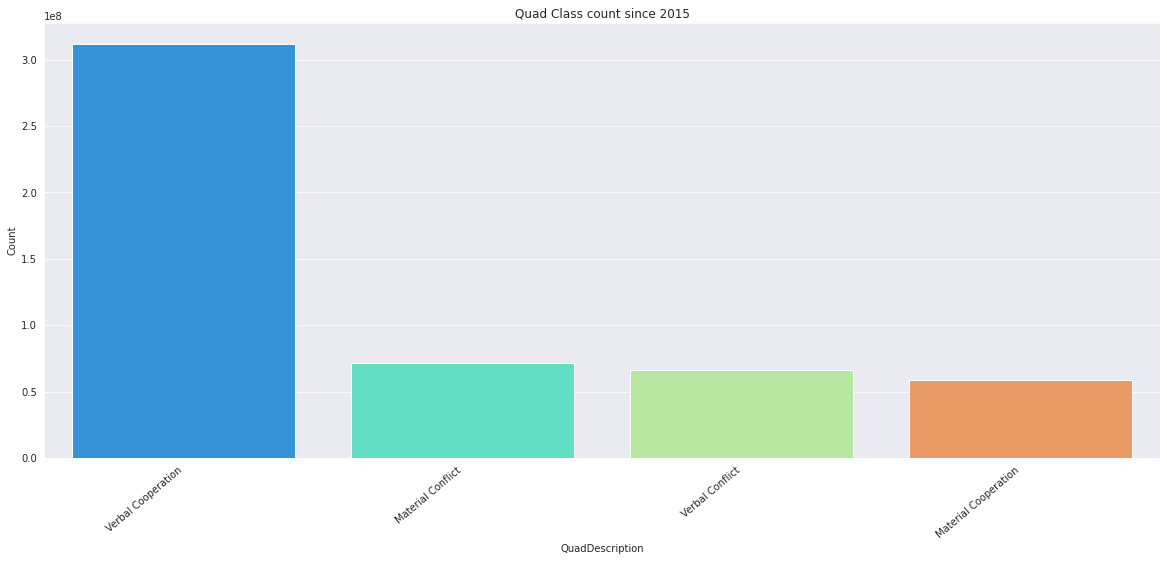
\includegraphics[width=1 \textwidth]{fig/GLOBAL/QC.png}
        \caption{Ilość zdarzeń dla poszczególnych kodów w czasie. (zródło: opracowanie własne)}
        \label{fig:GLOBALQC}
    \end{figure}

    \paragraph{Popularność czterokodów zdarzeń w czasie}
    Wykres~\ref{fig:GLOBALQCperc} przedstawia ilość zdarzeń dla czterokodów zdarzeń skumulowaną dla poszczególnych lat.
    WYKRES DO POPRAWY
    \begin{figure}[ht]
        \centering
        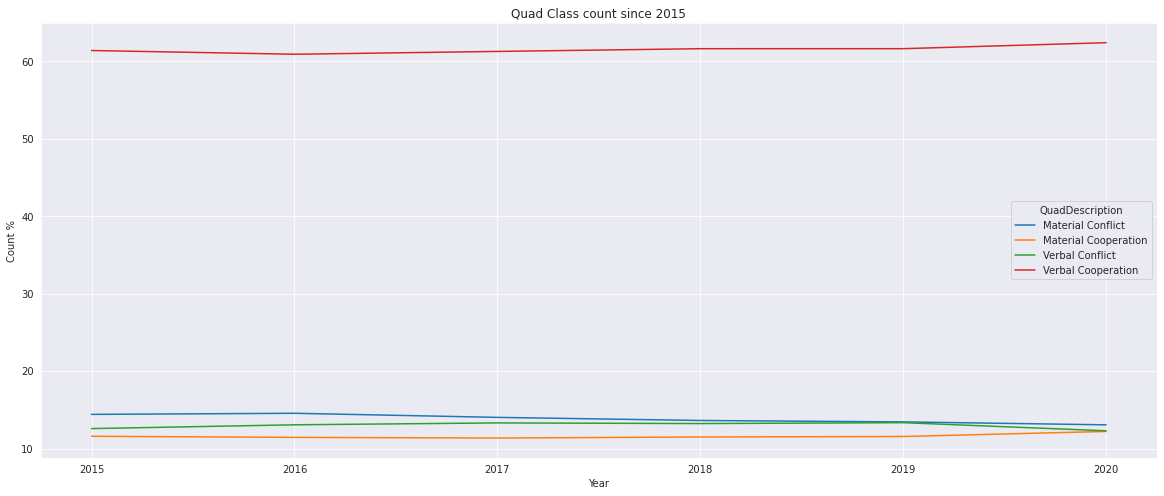
\includegraphics[width=1 \textwidth]{fig/GLOBAL/QCperc.png}
        \caption{Procentowa ilość zdarzeń dla poszczególnych kodów w czasie. (zródło: opracowanie własne)}
        \label{fig:GLOBALQCperc}
    \end{figure}

    \paragraph{Popularność bazowych kodów zdarzeń}
    Wykres~\ref{fig:GLOBALEBC} przedstawia sumaryczną ilość zdarzeń od 2015 roku, dla poszczególnych bazowych kodów zdarzeń, uszeregowaną malejąco.
    \begin{figure}[ht]
        \centering
        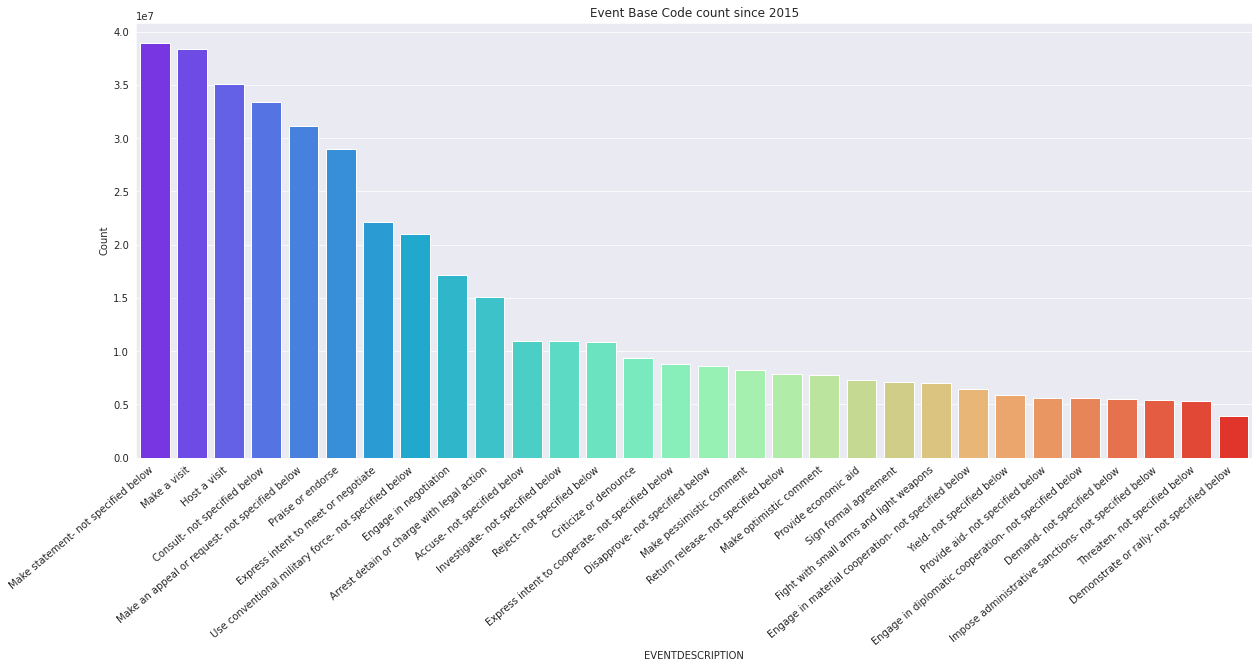
\includegraphics[width=1 \textwidth]{fig/GLOBAL/EBC.png}
        \caption{Ilość zdarzeń dla poszczególnych kodów w czasie. (zródło: opracowanie własne)}
        \label{fig:GLOBALEBC}
    \end{figure}

    \paragraph{Popularność bazowych kodów zdarzeń w czasie}
    Wykres~\ref{fig:GLOBALEBCperc} przedstawia ilość zdarzeń dla top 20 bazowych kodów zdarzeń skumulowaną dla poszczególnych lat.
    WYKRES DO POPRAWY
    \begin{figure}[ht]
        \centering
        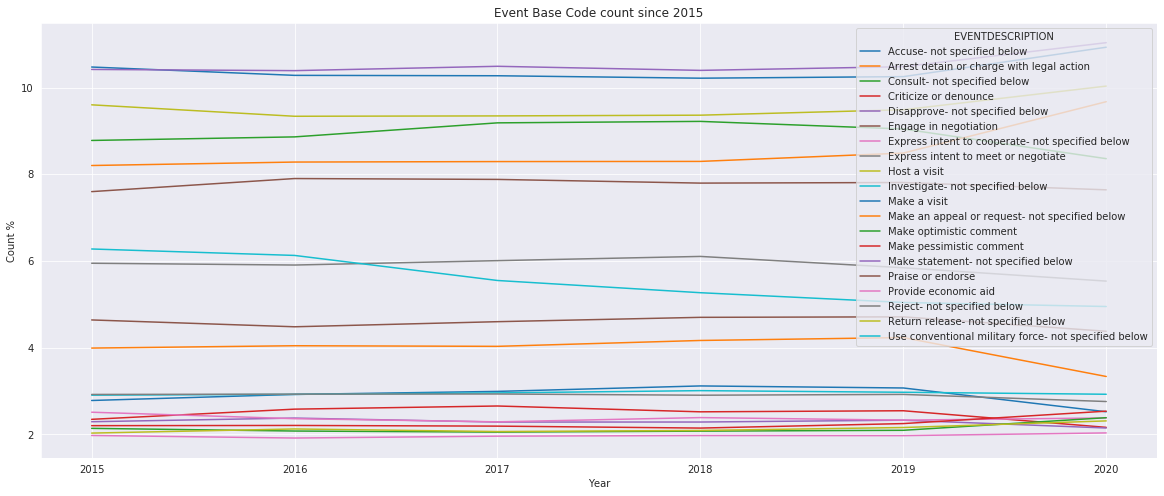
\includegraphics[width=1 \textwidth]{fig/GLOBAL/EBCperc.png}
        \caption{Procentowa ilość zdarzeń dla poszczególnych kodów w czasie. (zródło: opracowanie własne)}
        \label{fig:GLOBALEBCperc}
    \end{figure}

    \paragraph{Popularność podstawowych kodów zdarzeń}
    Wykres~\ref{fig:GLOBALERC} przedstawia sumaryczną ilość zdarzeń od 2015 roku, dla poszczególnych podstawowych kodów zdarzeń, uszeregowaną malejąco.
    \begin{figure}[ht]
        \centering
        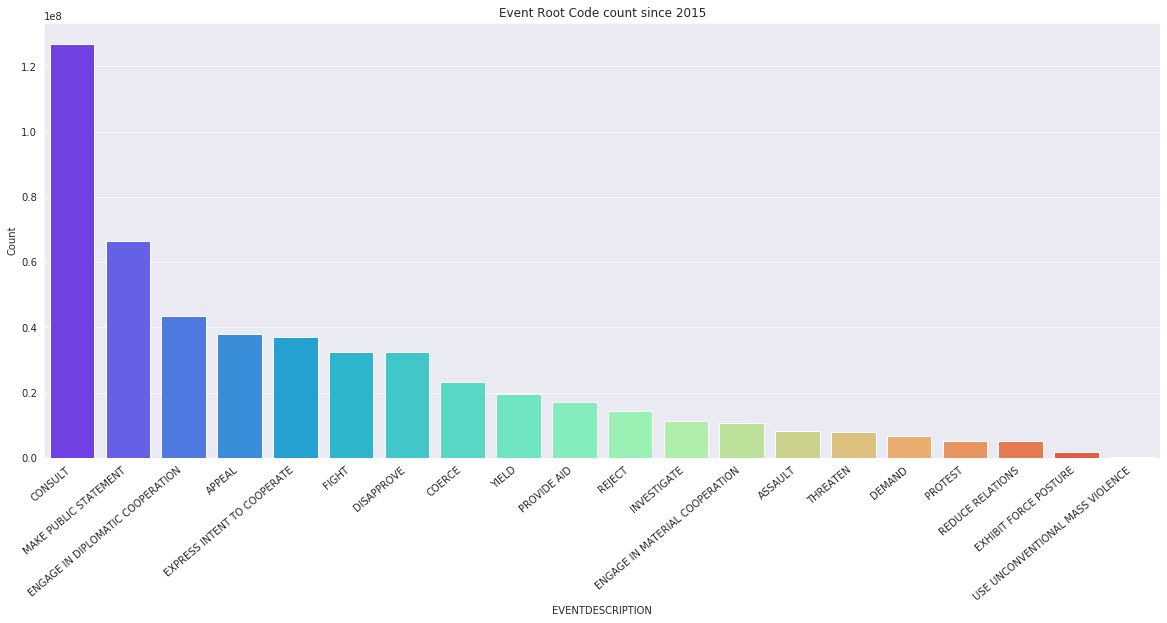
\includegraphics[width=1 \textwidth]{fig/GLOBAL/ERC.png}
        \caption{Ilość zdarzeń dla poszczególnych kodów w czasie. (zródło: opracowanie własne)}
        \label{fig:GLOBALERC}
    \end{figure}

    \paragraph{Popularność podstawowych kodów zdarzeń w czasie}
    Wykres~\ref{fig:GLOBALERCperc} przedstawia ilość zdarzeń dla top 20 podstawowych kodów zdarzeń skumulowaną dla poszczególnych lat.
    WYKRES DO POPRAWY
    \begin{figure}[ht]
        \centering
        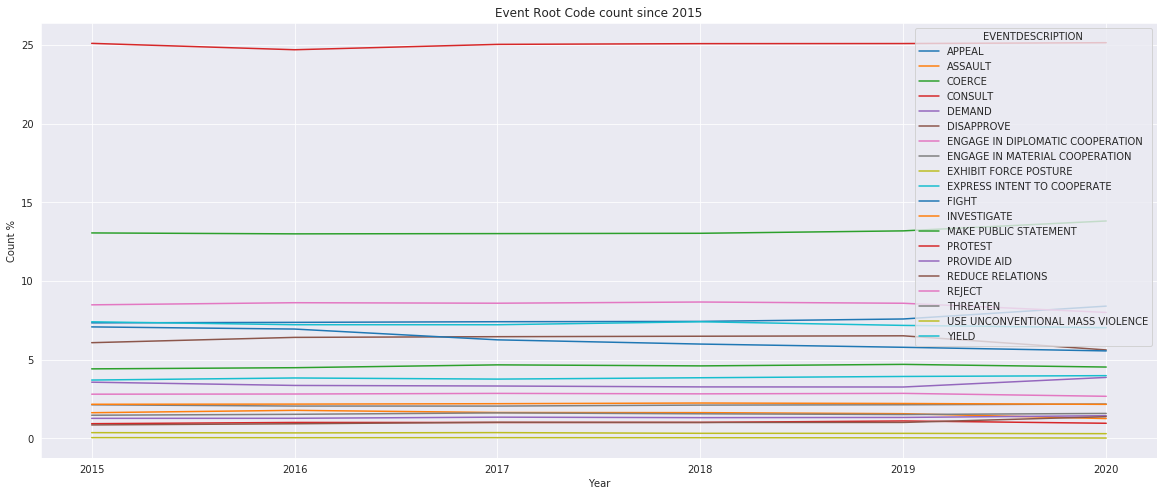
\includegraphics[width=1 \textwidth]{fig/GLOBAL/ERCperc.png}
        \caption{Procentowa ilość zdarzeń dla poszczególnych kodów w czasie. (zródło: opracowanie własne)}
        \label{fig:GLOBALERCperc}
    \end{figure}


    \section{Analiza danych dla wybranych krajów}

    \subsection{Polska}

    \paragraph{Kraj para do zdarzenia}


    Wykres~\ref{fig:PLpair} przedstawia ilość zdarzeń dla Polski w których parą jest dany kraj.

    \begin{figure}[ht]
        \centering
        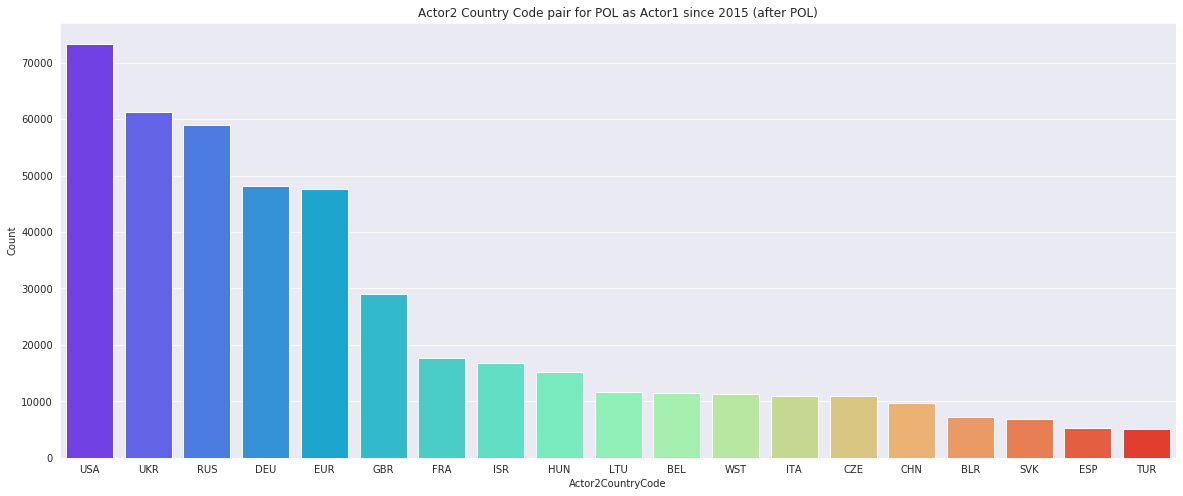
\includegraphics[width=1 \textwidth]{fig/PL/PLactor2Pair.png}
        \caption{Ilość zdarzeń w których parą jest dany kraj. (zródło: opracowanie własne)}
        \label{fig:PLpair}
    \end{figure}


    Wykres~\ref{fig:PLpairPerc} przedstawia ilość zdarzeń dla Polski w których parą jest dany kraj w czasie.

    WYKRES DO POPRAWY
    \begin{figure}[ht]
        \centering
        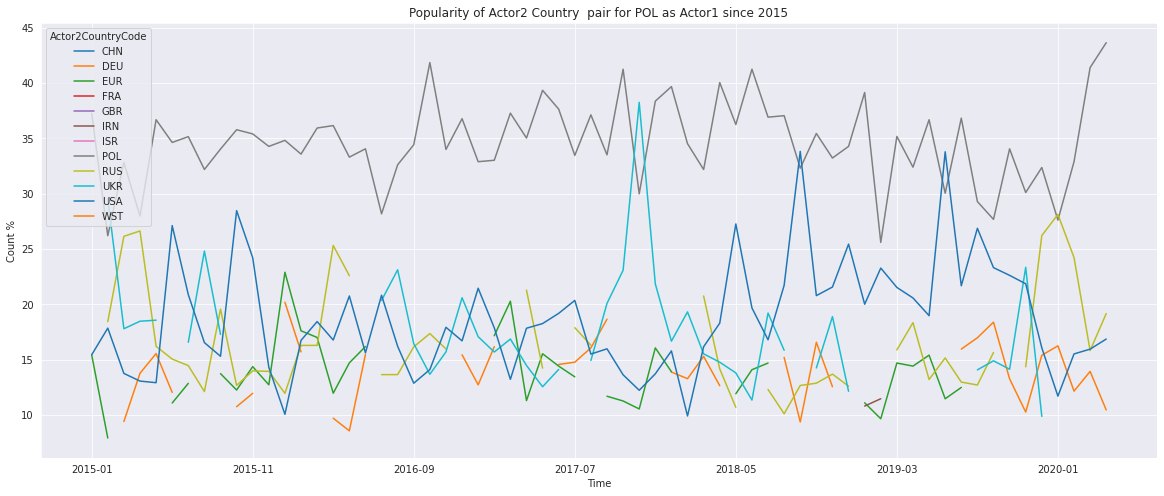
\includegraphics[width=1 \textwidth]{fig/PL/PLactor2PairPercinTIME.png}
        \caption{Procentowa ilość zdarzeń w których parą jest dany kraj w czasie. (zródło: opracowanie własne)}
        \label{fig:PLpairPerc}
    \end{figure}

    \paragraph{Podstawowy kod zdarzeń}

    Wykres~\ref{fig:PLPERC} przedstawia ilość zdarzeń dla Polski dla poszczególnych kodów podstawowych.


    \begin{figure}[ht]
        \centering
        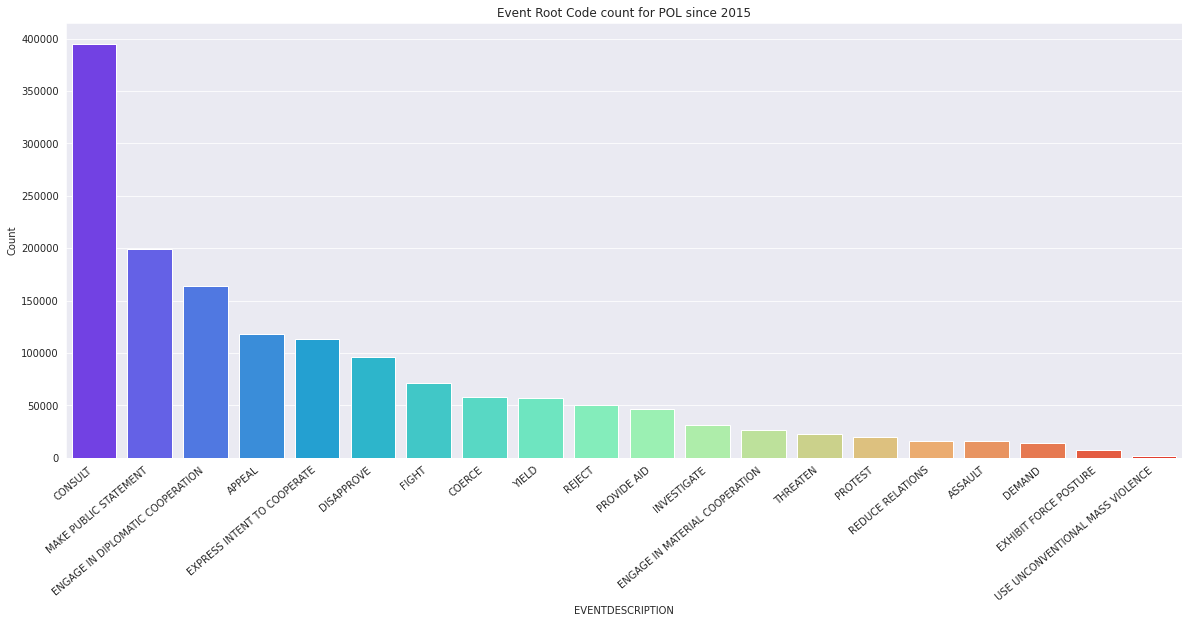
\includegraphics[width=1 \textwidth]{fig/PL/PLERC.png}
        \caption{Ilość zdarzeń dla poszczególnych kodów podstawowocy. (zródło: opracowanie własne)}
        \label{fig:PLPERC}
    \end{figure}

    Wykres~\ref{fig:PLPERCinTIME} przedstawia ilość zdarzeń dla Polski dla poszczególnych kodów podstawowych w czasie.

    WYKRES DO POPRAWY
    \begin{figure}[ht]
        \centering
        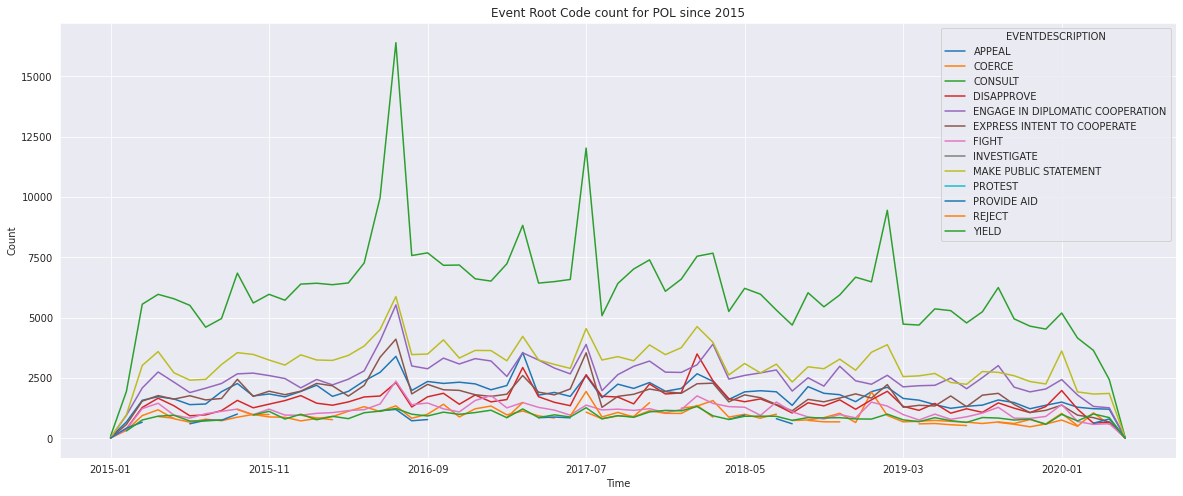
\includegraphics[width=1 \textwidth]{fig/PL/PLERCinTIME.png}
        \caption{Ilość zdarzeń dla poszczególnych kodów podstawowocy w czasie. (zródło: opracowanie własne)}
        \label{fig:PLPERCinTIME}
    \end{figure}

    Wykres~\ref{fig:PLPERCpercinTIME} przedstawia procentową ilość zdarzeń dla Polski dla poszczególnych kodów podstawowych w czasie.

    WYKRES DO POPRAWY
    \begin{figure}[ht]
        \centering
        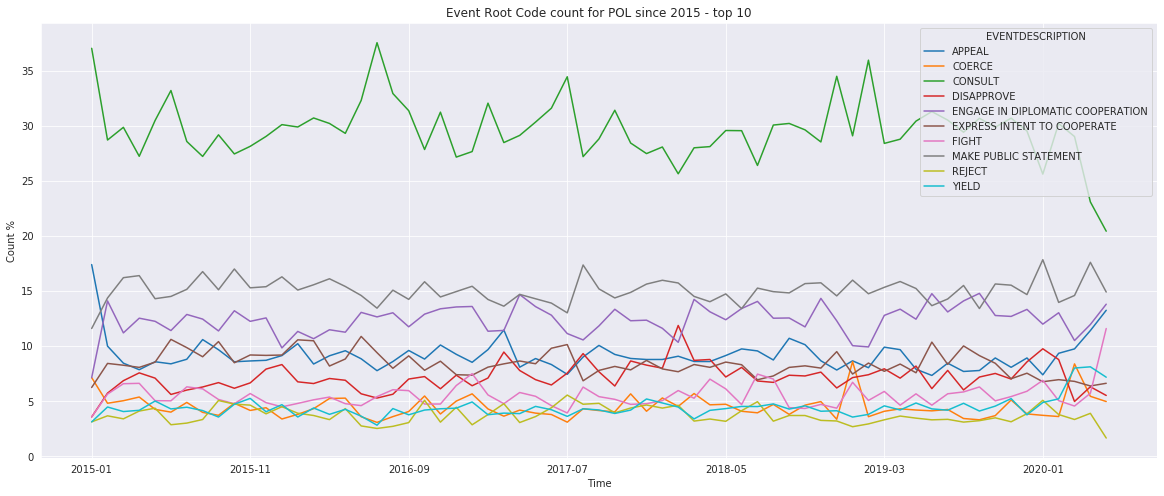
\includegraphics[width=1 \textwidth]{fig/PL/PLERCpercinTIME.png}
        \caption{Procentowa ilość zdarzeń dla poszczególnych kodów podstawowocy w czasie. (zródło: opracowanie własne)}
        \label{fig:PLPERCpercinTIME}
    \end{figure}

    \paragraph{Podstawowe kody zdarzeń między Polską a wybranymi krajami}

    Wykres~\ref{fig:PLDEUERC} przedstawia ilość zdarzeń z Niemcami dla poszczególnych kodów podstawowocy w czasie.

    WYKRES DO POPRAWY
    \begin{figure}[ht]
        \centering
        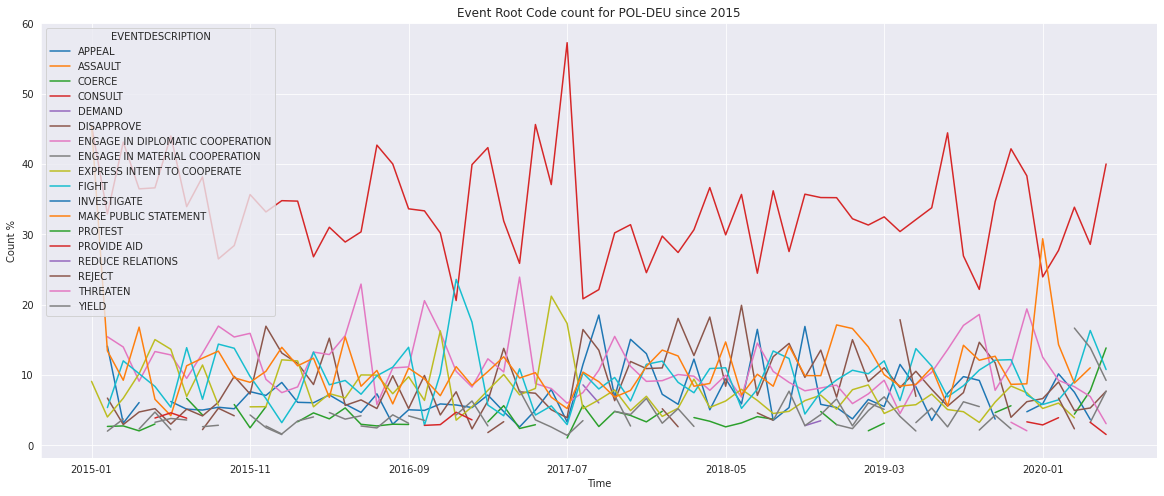
\includegraphics[width=1 \textwidth]{fig/PL/POLDEUERCperc.png}
        \caption{Procentowa ilość zdarzeń z Niemcami dla poszczególnych kodów podstawowocy w czasie. (zródło: opracowanie własne)}
        \label{fig:PLDEUERC}
    \end{figure}

    Wykres~\ref{fig:PLFRAERC} przedstawia ilość zdarzeń z Francją dla poszczególnych kodów podstawowocy w czasie.


    WYKRES DO POPRAWY
    \begin{figure}[ht]
        \centering
        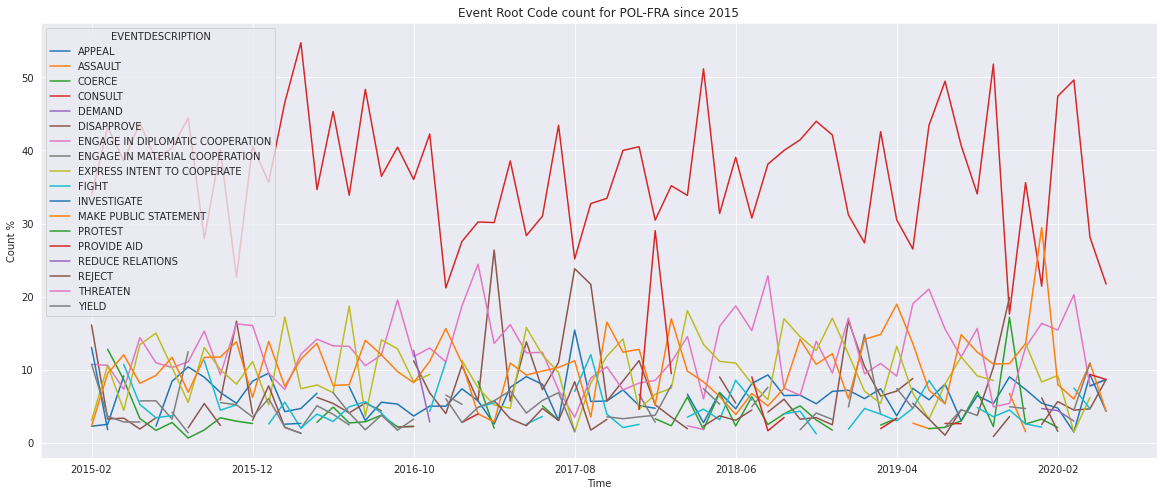
\includegraphics[width=1 \textwidth]{fig/PL/POLFRAERCperc.png}
        \caption{Procentowa ilość zdarzeń z Francją dla poszczególnych kodów podstawowocy w czasie. (zródło: opracowanie własne)}
        \label{fig:PLFRAERC}
    \end{figure}

    Wykres~\ref{fig:PLGBRERC} przedstawia ilość zdarzeń z Wielką Brytanią dla poszczególnych kodów podstawowocy w czasie.

    WYKRES DO POPRAWY
    \begin{figure}[ht]
        \centering
        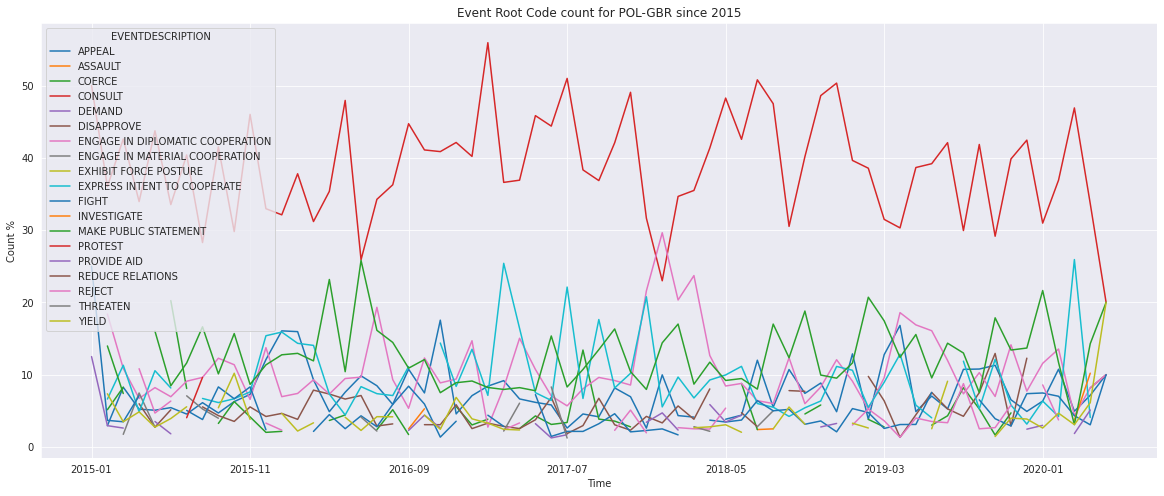
\includegraphics[width=1 \textwidth]{fig/PL/POLGBRERCperc.png}
        \caption{Procentowa ilość zdarzeń z Wielka Brytanią dla poszczególnych kodów podstawowocy w czasie. (zródło: opracowanie własne)}
        \label{fig:PLGBRERC}
    \end{figure}

    Wykres~\ref{fig:PLRUSERC} przedstawia ilość zdarzeń z Rosją dla poszczególnych kodów podstawowocy w czasie.

    WYKRES DO POPRAWY
    \begin{figure}[ht]
        \centering
        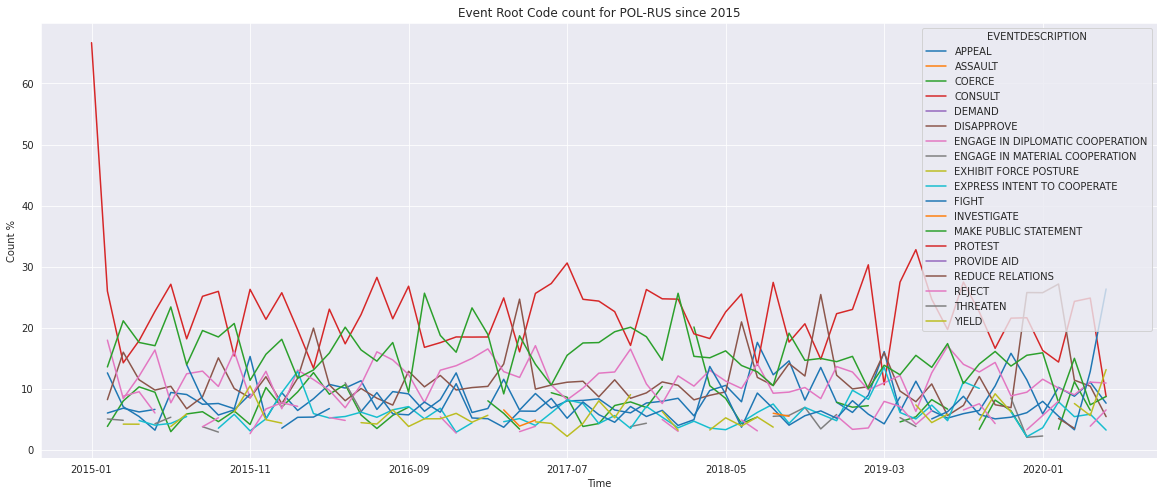
\includegraphics[width=1 \textwidth]{fig/PL/POLRUSERCperc.png}
        \caption{Procentowa ilość zdarzeń z Rosją dla poszczególnych kodów podstawowocy w czasie. (zródło: opracowanie własne)}
        \label{fig:PLRUSERC}
    \end{figure}

    \subsection{Niemcy}

    \subsection{Rosja}

    \subsection{Stan zjednoczone}

    \subsection{Pozostałe}


    \section{Analiza siły powiązania}

    \subsection{Analiza siły powiązania miedzy wybranymi krajami}

    \paragraph{Polska}

    Wykres~\ref{fig:PLConnection} przedstawia siłę połączenia Polski z wybranaymi krajami w czasie.


    \begin{figure}[ht]
        \centering
        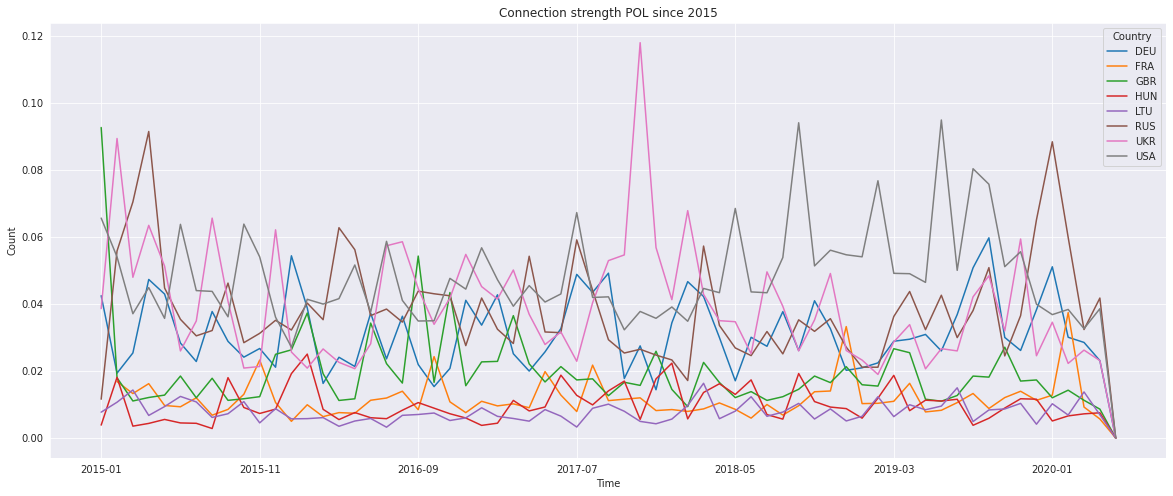
\includegraphics[width=1 \textwidth]{fig/PL/POLConnection.png}
        \caption{Siła połączenia Polski z wybranymi krajami w czasie. (zródło: opracowanie własne)}
        \label{fig:PLConnection}
    \end{figure}

    \paragraph{Rosja}

    Wykres~\ref{fig:RUSConnection} przedstawia siłę połączenia Rosji z wybranaymi krajami w czasie.

    \begin{figure}[ht]
        \centering
        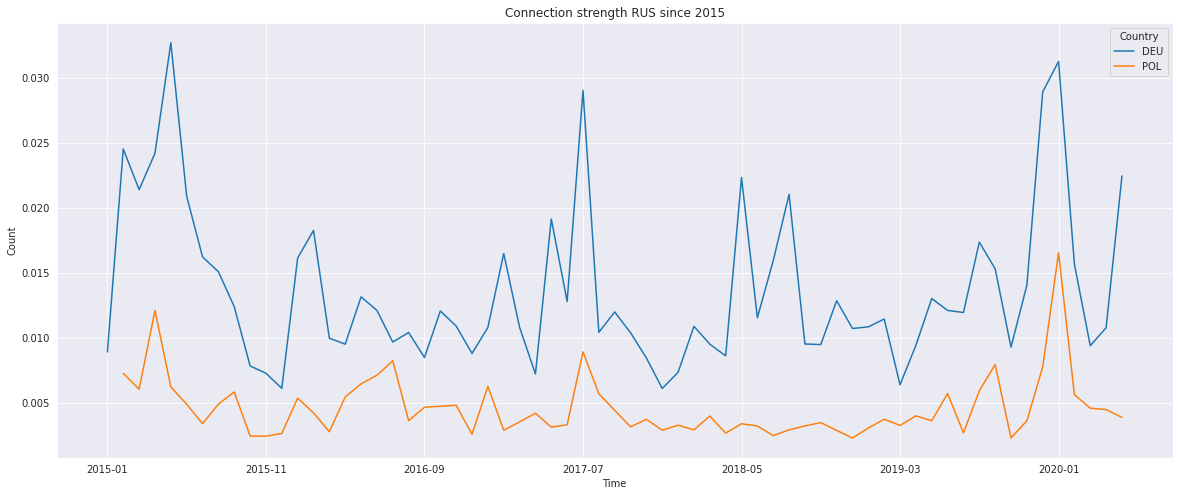
\includegraphics[width=1 \textwidth]{fig/RUS/RUSConnection.png}
        \caption{Siła połączenia Rosji z wybranymi krajami w czasie. (zródło: opracowanie własne)}
        \label{fig:RUSConnection}
    \end{figure}

    \paragraph{Niemcy}

    Wykres~\ref{fig:DEUConnection} przedstawia siłę połączenia Niemiec z wybranaymi krajami w czasie.

    \begin{figure}[ht]
        \centering
        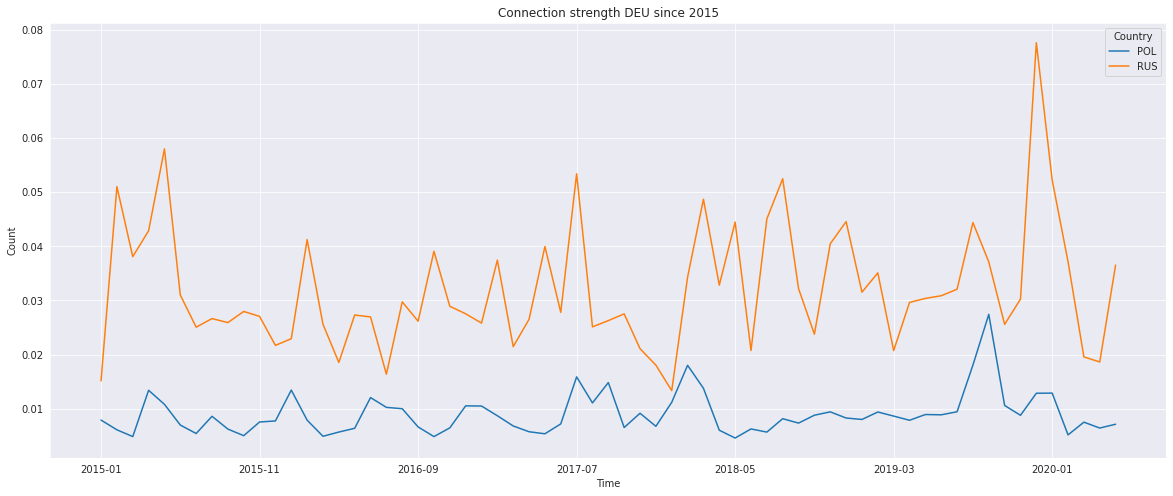
\includegraphics[width=1 \textwidth]{fig/DEU/DEUConnection.png}
        \caption{Siła połączenia Niemiec z wybranymi krajami w czasie. (zródło: opracowanie własne)}
        \label{fig:DEUConnection}
    \end{figure}

    \paragraph{Stany Zjednoczone}

    Wykres~\ref{fig:PLConnection} przedstawia siłę połączenia Stanów Zjednoczonych z wybranaymi krajami w czasie.

    \begin{figure}[ht]
        \centering
        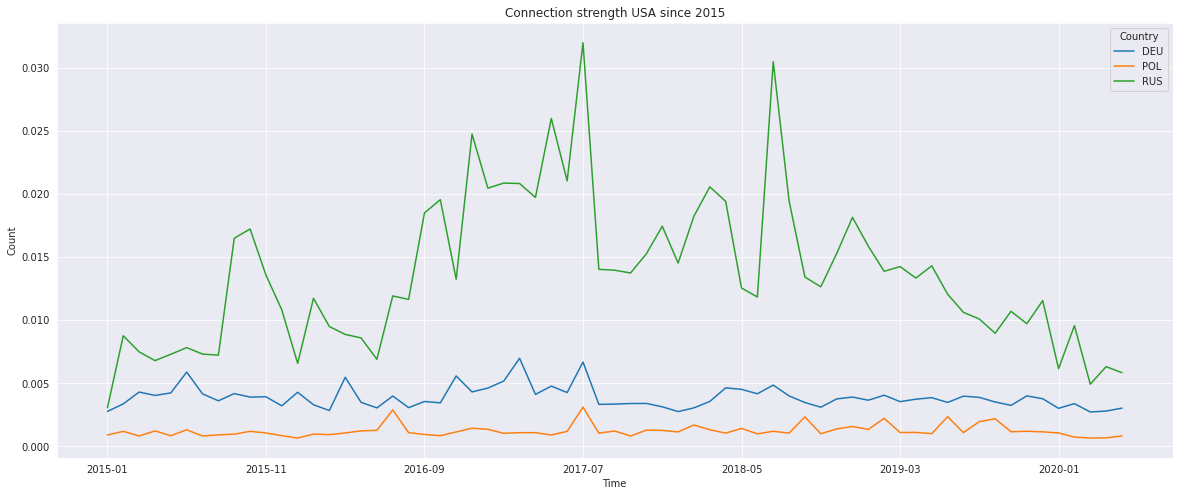
\includegraphics[width=1 \textwidth]{fig/USA/USAConnection.png}
        \caption{Siła połączenia Stanów Zjednoczonych z wybranymi krajami w czasie. (zródło: opracowanie własne)}
        \label{fig:USAConnection}
    \end{figure}

    \subsection{Analiza symetryczności siły powiązania}

    \paragraph{Polska - Niemcy - Polska}

    Wykres~\ref{fig:POL-DEU-POL} przedstawia symetryczność siły połączenia Polski i Niemiec w czasie.


    \begin{figure}[ht]
        \centering
        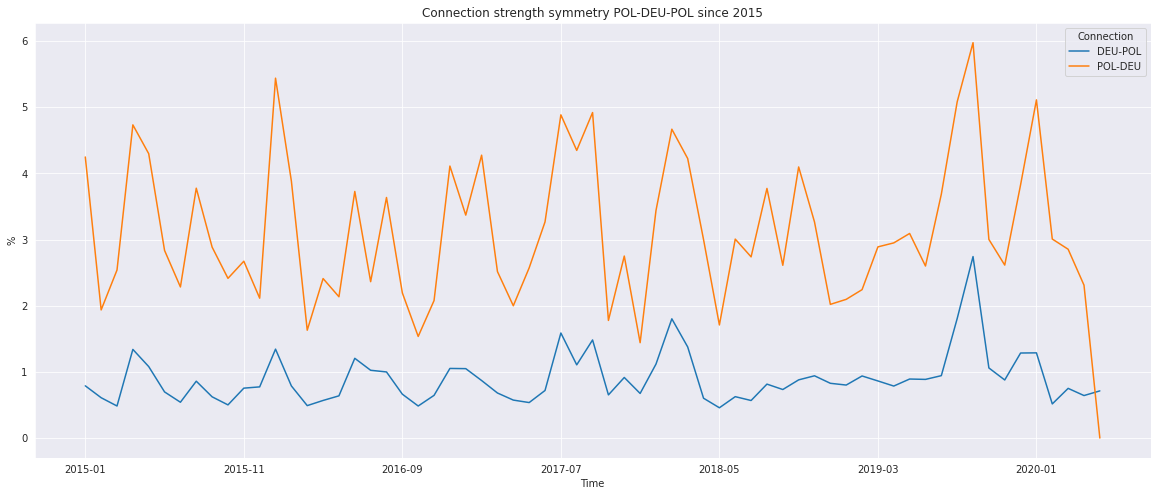
\includegraphics[width=1 \textwidth]{fig/ConnectionSymmetry/POL-DEU-POL.png}
        \caption{Symetryczność siły połączenia Polski i Niemiec w czasie. (zródło: opracowanie własne)}
        \label{fig:POL-DEU-POL}
    \end{figure}

    \paragraph{Polska - Rosja - Polska}

    Wykres~\ref{fig:POL-RUS-POL} przedstawia symetryczność siły połączenia Polski i Rosji w czasie.


    \begin{figure}[ht]
        \centering
        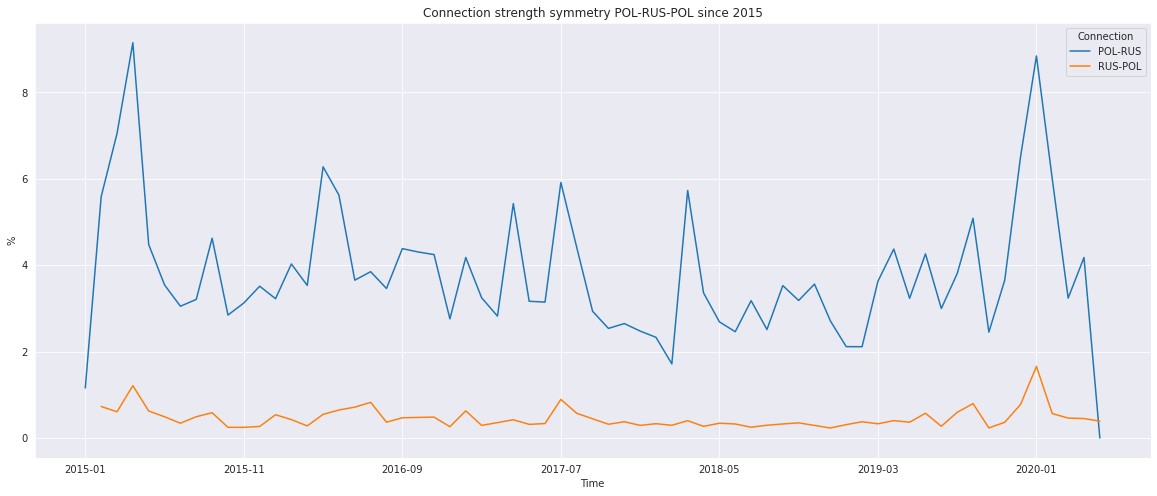
\includegraphics[width=1 \textwidth]{fig/ConnectionSymmetry/POL-RUS-POL.png}
        \caption{Symetryczność siły połączenia Polski i Rosji w czasie. (zródło: opracowanie własne)}
        \label{fig:POL-RUS-POL}
    \end{figure}

    \paragraph{Polska - Stany Zjednoczone - Polska}

    Wykres~\ref{fig:POL-USA-POL} przedstawia symetryczność siły połączenia Polski i Stanów Zjednoczonych w czasie.


    \begin{figure}[ht]
        \centering
        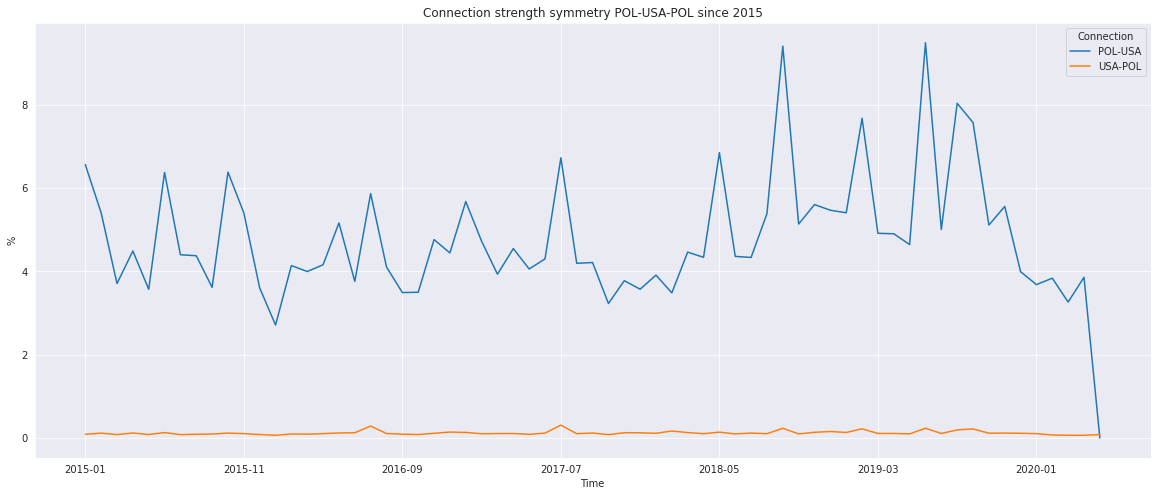
\includegraphics[width=1 \textwidth]{fig/ConnectionSymmetry/POL-USA-POL.png}
        \caption{Symetryczność siły połączenia Polski i Stanów Zjednoczonych w czasie. (zródło: opracowanie własne)}
        \label{fig:POL-USA-POL}
    \end{figure}


    \section{Analiza wybranych kodów podstawowych}

    \subsection{Fight}

    Wykres~\ref{fig:Fight} przedstawia procentową ilość państw z jakimi dany kraj ma zdarzenia fight w czasie.


    \begin{figure}[ht]
        \centering
        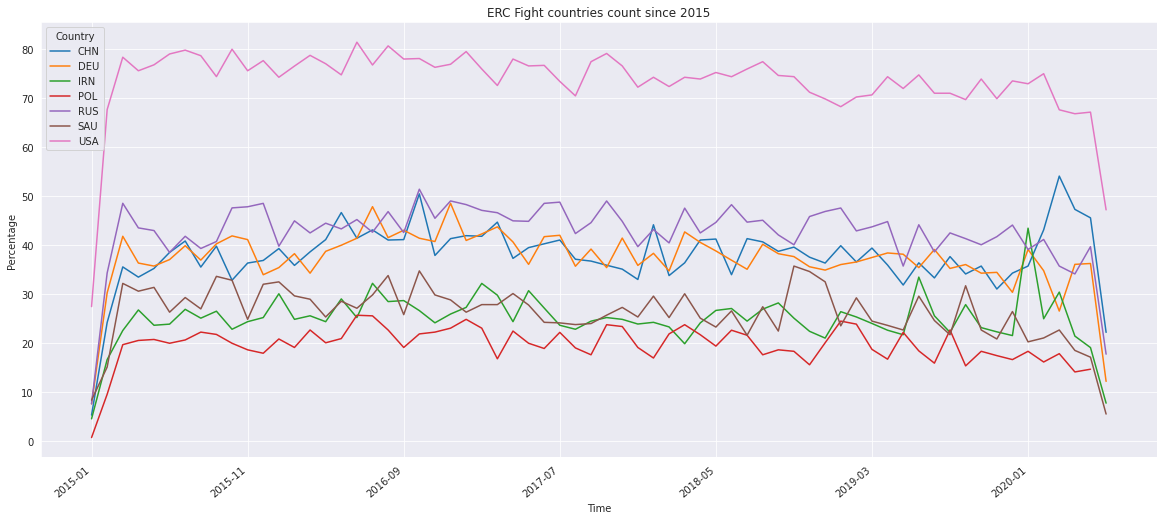
\includegraphics[width=1 \textwidth]{fig/ERC/Fight.png}
        \caption{Procentowa ilość państw z jakimi dany kraj ma zdarzenia fight w czasie. (zródło: opracowanie własne)}
        \label{fig:Fight}
    \end{figure}

    \subsection{Express intent to cooperate}

    Wykres\ldots przedstawia procentową ilość państw z jakimi dany kraj ma zdarzenia fight w czasie.


    \section{Analiza średniego tonu wydarzeń dla wybranych krajów}


    \section{Analiza miary Goldsteina wydarzeń dla wybranych krajów}


    \section{Klasteryzacja}

    \subsection{A}

    Do przeprowadzenia pierwszego grupowania krajów wykorzystany został wektor składający się z:
    \begin{enumerate}
        \item[•] ilości zdarzeń dla których kraj jest aktorem 1
        \item[•] ilości wzmianek (numMentions)
        \item[•] ilości material conflict/cooperation z quad description
        \item[•] ilości verbal conflict/cooperation z quad description
        \item[•] średniego średniego tonu
        \item[•] średniej miary Goldsteina
        \item[•] ilości zdarzeń Fight
        \item[•] ilości zdarzeń Express intent to cooperate
    \end{enumerate}
    Dane wykorzystane w tym doświadczeniu pochodzą ze stycznia 2020 roku.


    \chapter{Podsumowanie}
    W niniejszej części zostaną opisane wnioski z pracy według kolejności wcześniej przedstawionych rozdziałów.


    \section{Dalsze kierunki rozwoju}
    W tej części zostaną opisane możliwe kierunki rozwoju pracy.

    \paragraph{Analiza pod kątem COVID-19}

    \paragraph{Analiza pod kątem grup etnicznych}

    \paragraph{Analiza pod kątem grup religijnych}


    \inputencoding{utf8}

    \newpage
    \addcontentsline{toc}{chapter}{Bibliografia}
    \printbibliography[title={Bibliografia}]

\end{document}
